\chapter{Algorithm Implementation and Operational Workflows}
\label{chap:ch4}

\par This chapter describes in detail the concrete implementation of every major operational flow in the QuickShift system. Beyond the core scheduling engine, the platform manages a full lifecycle of workforce events: leave requests submitted by employees, absence reports that trigger automated replacement searches, manual corrections made by managers, and the complete notification loop that connects all participants. Each of these workflows is underpinned by the same constraint-satisfaction principles used in the scheduler, ensuring behavioral consistency across the system.

%===========================================================
\section{Automated Schedule Generation}
\label{sec:automated_schedule_generation}
%===========================================================

\subsection{Input data and preprocessing}
\par Every scheduling run begins with a data ingestion step. The backend reads a structured Excel file that contains one row per working day, carrying at minimum a date, a projected daily sales figure, and a boolean flag indicating whether a merchandise reception is expected on that day. The reading is performed by a dedicated \texttt{CsvReaderService} and the output is a typed list of \texttt{DayForecastDto} objects, each encapsulating the complete context needed for a single day of scheduling.

\par The target month is resolved to the next calendar month automatically. This design keeps the scheduling endpoint simple for the most common use case while still supporting the Leave Request functionality, by only allowing employees to request leave with at least 1 month prior. In this way we make sure that the schedule does not shift as much with only a few days before the month's beginning, and therefore it does not confuse the employees with massive changes on short notice.

\par For deployments serving multiple stores, the forecast Excel can be organized into named sheets, each corresponding to a store. The backend accepts an optional store identifier which is translated into a sheet name via the \texttt{Store} entity. If no matching sheet is found or the resulting row set for the requested month is empty, the generation is aborted early and a clear error is returned to the caller. This prevents silently producing an empty or partial schedule when input data is missing.

\subsection{Schedule generation pipeline}
\par The overall generation flow is structured as a deterministic pipeline that processes the forecast list sequentially. Before computing any new assignments, the system retrieves all existing shifts for the target month and store from the database. If any exist, they are removed together with their linked absence requests and replacement offers, ensuring that the regenerated schedule is always internally consistent and does not contain residual data from a previous run.

\par This delete-before-generate strategy is a deliberate architectural choice. An alternative approach would be to compute a diff between the old and new schedules and apply only the changes. While that would produce smaller database operations, it introduces significant complexity in handling the intermediate states of absence requests and replacement chains that may reference old shifts. The chosen approach trades a slightly larger write at generation time for a dramatically simpler consistency model, which is more appropriate for the operational scale of the target deployment.

\par After the cleanup phase, employee trackers are initialized for all employees in scope, and the algorithm iterates day by day through the forecast list. At the end of the loop, all produced shift objects are persisted in bulk using a single \texttt{saveAll} call, which keeps the transaction boundary short and avoids partial writes.

\subsection{The Constraint Model}
\par The solver enforces two categories of constraints. Hard constraints represent legal or operational limits that must hold unconditionally for any produced schedule:

\begin{itemize}
    \item \textbf{Maximum consecutive working days}: no employee may work more than five days in a row. Once this limit is reached, the employee is excluded from candidate selection until a day off is registered.
    \item \textbf{12-hour back-to-back prohibition}: an employee who worked a 12-hour shift on the previous day is excluded from the following day's assignment, regardless of weekly hour accumulation.
    \item \textbf{Weekly hour caps}: the maximum number of hours assignable in a single calendar week depends on contract type. Full-time employees (8-hour contracts) may not exceed 40 hours per week; employees on a 6-hour part-time contract are capped at 30 hours; employees on a 4-hour contract are capped at 20 hours per week.
    \item \textbf{Approved leave}: employees with an approved leave request covering the target day are completely excluded from candidate selection for that day.
\end{itemize}

\par Soft constraints guide candidate ranking when multiple legal candidates exist. The primary soft rule is shift preference: employees who have declared a preference for morning or evening shifts are ranked above equally eligible candidates with a different preference or no declared preference. The secondary soft rule is monthly hour balance: among candidates with the same preference score, the one with the fewest accumulated hours in the current month is preferred. Together, these two soft rules produce schedules that are both preference-aligned and balanced without requiring a dedicated optimization pass. Technically speaking, this is the \textbf{true game-changer for QuickShift}. While other tools available on the market design basic end-to-end shifts that only take into account the hard constraints, this application truly takes into consideration what the employee prefers, therefore significantly raising the quality of work produced. All this is done in parallel with the forecast functionality, achieving a balance between the quality of life and productivity for the employee.

\subsection{Coverage scaling from forecast signals}
\par The default staffing target is one employee per time window (morning and evening), for a daily total of two employees.

Several business rules are used to adjust staffing requirements. First, the weekend effect accounts for the fact that Saturday and Sunday are inherently high-traffic days in retail. Therefore, the minimum staffing level for both the morning and evening slots is raised to two employees, resulting in a daily total of four employees.

Similarly, on a reception day, when a merchandise shipment is expected, additional staff are required to unload and process stock. As a result, the minimum staffing level for both slots is also raised to two employees.

The day before reception is subject to the same elevated staffing requirements because preparation work must be carried out in anticipation of the incoming shipment.

Sales projections also influence staffing levels. Under the big sales threshold rule, if the projected daily sales exceed a configurable threshold (currently set to 2,000 monetary units), one additional employee is assigned to the evening slot to accommodate increased customer traffic during peak afternoon hours.

Finally, the massive sales threshold rule applies when projected sales exceed a higher threshold (currently 5,000 monetary units). In this case, an additional employee is assigned to the morning slot as well, reflecting the needs of exceptional commercial events such as national holidays or promotional campaigns.

\par These thresholds are defined as instance fields in the scheduling service and can be adjusted without modifying the algorithm logic. The design makes the coverage model transparent and tunable by someone with domain knowledge, without requiring code changes.

\subsection{Heuristic solver and the employee tracker}
\par The solver is built on a greedy heuristic enhanced by a stateful per-employee tracking structure called \texttt{EmployeeTracker}. Each tracker wraps an \texttt{Employee} entity and maintains three pieces of mutable state:

\begin{figure}[h!]
    \centering
    \begin{tikzpicture}[
        node distance=1.5cm and 1.5cm,
        mainbox/.style={rectangle, draw=blue!70, thick, fill=blue!5, text width=3.5cm, align=center, rounded corners=1ex, minimum height=1.2cm, font=\sffamily\bfseries},
        metricbox/.style={rectangle, draw=black!70, thick, fill=gray!5, text width=5cm, align=left, rounded corners=1ex, minimum height=1cm, font=\sffamily\small},
        limitbox/.style={rectangle, draw=red!60, thick, fill=red!5, text width=3.5cm, align=left, rounded corners=1ex, minimum height=0.6cm, font=\sffamily\footnotesize},
        arrow/.style={thick, ->, >=stealth, draw=black!70},
        dashedarrow/.style={thick, ->, >=stealth, draw=red!70, dashed}
    ]

    % Main Engine Node
    \node (engine) [mainbox] {Algorithm \\ Tracking Engine};

    % Metric Nodes
    \node (weekly) [metricbox, right=1.5cm of engine] {\textbf{Weekly Hours} \\ Cumulative ISO week total};
    \node (monthly) [metricbox, above=0.8cm of weekly] {\textbf{Monthly Hours} \\ Cumulative month total};
    \node (consecutive) [metricbox, below=0.8cm of weekly] {\textbf{Consecutive Days} \\ Unbroken sequence counter};

    % Reset/Limit Nodes
    \node (rmonthly) [limitbox, right=1cm of monthly] {Reset: 1st of Month};
    \node (rweekly) [limitbox, right=1cm of weekly] {Reset: Every Monday};
    \node (rconsecutive) [limitbox, right=1cm of consecutive] {Limit: 5 Days \\ Reset: Day-Off};

    % Arrows from Engine to Metrics
    \draw [arrow] (engine.east) -- ++(0.5,0) |- (monthly.west);
    \draw [arrow] (engine.east) -- (weekly.west);
    \draw [arrow] (engine.east) -- ++(0.5,0) |- (consecutive.west);

    % Arrows from Metrics to Limits
    \draw [dashedarrow] (monthly.east) -- (rmonthly.west);
    \draw [dashedarrow] (weekly.east) -- (rweekly.west);
    \draw [dashedarrow] (consecutive.east) -- (rconsecutive.west);

    \end{tikzpicture}
    \caption{Internal metric tracking and constraint triggers utilized by the scheduling algorithm.}
    \label{fig:algorithm_tracking}
\end{figure}

\par On each day, the solver computes the total number of employee slots to fill and iterates through them in order. For each slot it determines whether the next assignment must be a morning or evening shift, and whether it is the first assignment of that slot (which requires a full-time employee to maintain service quality). Candidates are sorted by least monthly hours before preference matching is attempted, so the greedy selection naturally distributes hours across the team over the course of the month.

\par The selection itself proceeds in two passes. The first pass looks only at candidates whose declared preference matches the required slot. If such a candidate exists and satisfies all hard constraints, they are selected immediately. If the first pass finds no match, a second fallback pass selects the legally available candidate with the smallest amount of hours worked in that specific month, regardless of preference. This two-pass design avoids sacrificing coverage when no preferred candidate is available, while still honoring preferences whenever they do not conflict with operational needs.

\subsection{Shift proposal generation and contract mapping}
\par Once a candidate is selected, the system generates a concrete shift proposal based on their contract type and the required time window. The mapping is as follows:

\begin{table}[h]
\centering
\caption{Shift mapping by contract type and slot}
\begin{tabular}{|l|l|l|}
\hline
\textbf{Contract Type} & \textbf{Morning Slot} & \textbf{Evening Slot} \\ \hline
\texttt{FULL\_TIME\_8H} 
& \texttt{SHIFT\_1\_10\_18} (10:00--18:00) 
& \texttt{SHIFT\_2\_14\_22} (14:00--22:00) \\ \hline

\texttt{PART\_TIME\_6H} 
& \texttt{PART\_TIME\_10\_16} 
& \texttt{PART\_TIME\_16\_22} \\ \hline

\texttt{PART\_TIME\_4H} 
& \texttt{PART\_TIME\_10\_14} 
& \texttt{PART\_TIME\_16\_20} \\ \hline
\end{tabular}
\label{tab:shift_mapping}
\end{table}

\par Each proposal carries the shift type string, the duration in hours, and a boolean indicating whether it falls in the morning window. The duration is used immediately for the weekly hour check before the candidate is accepted, preventing over-assignment at the point of selection rather than as a post-processing correction.

%===========================================================
\section{Absence and Replacement Workflows}
\label{sec:absence_and_replacement_workflows}
%===========================================================

\subsection{The absence reporting flow}
\par Employees frequently need to report that they cannot attend a scheduled shift on short notice. The system provides a structured absence reporting mechanism that initiates a formal workflow rather than relying on informal communication between the employee and the manager.

\par When an employee submits an absence report through the frontend, the backend validates several preconditions before accepting it:

\begin{itemize}

    \item The shift must belong to the requesting employee (ownership verification).

    \item The shift date must be strictly in the future — past shifts cannot be reported.

    \item The shift must be in a reportable state: both \texttt{SCHEDULED} and \texttt{REPLACEMENT} shifts are eligible, but a shift that has already been marked \texttt{ABSENT} or is in another terminal state is rejected.

    \item There must not already be a pending absence request for the same shift, preventing duplicate submissions.

\end{itemize} 


\par If all checks pass, an \texttt{AbsenceRequest} entity is persisted with status \texttt{PENDING}, and a notification is sent to the store manager. The notification message follows a structured format prefixed with \texttt{[ABSENCE REQUEST]}, which allows the frontend to identify the notification type and render the appropriate action control. The notification carries a reference to the absence request ID, linking the notification to the workflow object without duplicating data.

\subsection{Manager acknowledgment and the replacement algorithm}
\par Upon receiving an absence notification, the manager can acknowledge the request directly from the notifications page. Acknowledgment triggers a multi-step process:

\vspace{1.5em}
\begin{figure}[!h]
    \centering
    \begin{tikzpicture}[
        node distance=0.8cm,
        startbox/.style={rectangle, draw=blue!70, thick, fill=blue!5, text width=7.5cm, align=center, rounded corners=1ex, minimum height=0.8cm, font=\sffamily\bfseries},
        actionbox/.style={rectangle, draw=black!70, thick, fill=gray!5, text width=7.5cm, align=left, rounded corners=1ex, minimum height=0.9cm, font=\sffamily\small},
        decisionbox/.style={diamond, aspect=2.5, draw=orange!70, thick, fill=orange!5, text width=4.5cm, align=center, font=\sffamily\small\bfseries},
        deductbox/.style={rectangle, draw=red!70, thick, fill=red!5, text width=4cm, align=center, rounded corners=1ex, minimum height=0.8cm, font=\sffamily\small},
        enginebox/.style={rectangle, draw=purple!70, thick, fill=purple!5, text width=7.5cm, align=center, rounded corners=1ex, minimum height=0.9cm, font=\sffamily\bfseries},
        arrow/.style={thick, ->, >=stealth, draw=black!70}
    ]

    % Nodes
    \node (start) [startbox] {Absence Request Approved};
    
    \node (step1) [actionbox, below=0.8cm of start] {\textbf{1. State Update} \\ Original shift marked as \texttt{ABSENT}. Visible on public calendar.};
    
    \node (step2) [decisionbox, below=0.8cm of step1] {Was it a regular \\ (non-replacement) shift?};
    
    \node (deduct) [deductbox, right=1cm of step2] {\textbf{2. Leave Deduction} \\ Decrement balance by 1};
    
    \node (step3) [enginebox, below=1cm of step2] {\textbf{3. Replacement Finder Engine} \\ System searches for the optimal available substitute};

    % Arrows
    \draw [arrow] (start) -- (step1);
    \draw [arrow] (step1) -- (step2);
    
    % Decision branch: YES
    \draw [arrow] (step2.east) -- node[above, font=\sffamily\footnotesize] {Yes} (deduct.west);
    \draw [arrow] (deduct.south) |- (step3.east);
    
    % Decision branch: NO
    \draw [arrow] (step2.south) -- node[right, font=\sffamily\footnotesize] {No} (step3.north);

    \end{tikzpicture}
    \caption{Automated system workflow triggered upon reporting a shift absence.}
    \label{fig:absence_processing_workflow}
\end{figure}
\vspace{1.5em}

\par The replacement finder reconstructs the full scheduling state for the target month before making its selection. It loads all shifts for the store from the beginning of the month up to and including the absence date, then replays them day by day through \texttt{EmployeeTracker} instances. This replay ensures that the replacement search respects the same constraints as the original scheduler: weekly hours are tracked correctly across ISO week boundaries, consecutive day counts are accurate, and no candidate is selected who would violate a hard constraint as a result of the replacement assignment.

\par After the replay, the finder applies the following eligibility filters to the candidates:

\vspace{1.5em}
\begin{table}[h!]
    \centering
    \caption{Algorithmic constraints evaluated by the replacement finder engine.}
    \renewcommand{\arraystretch}{1.5}
    \begin{tabular}{|l|p{4.5cm}|p{6cm}|}
        \hline
        \textbf{Domain} & \textbf{Constraint Metric} & \textbf{Algorithmic Application} \\ \hline
        \multirow{2}{*}{\textbf{Availability}} & Not Already Scheduled & Rejects candidates who already possess an assigned shift on the target date. \\ \cline{2-3}
        & Not on Approved Leave & Cross-references the leave database; excludes employees on official vacation. \\ \hline
        \multirow{2}{*}{\textbf{Fatigue \& Rest}} & Consecutive Days Limit & Evaluates trailing schedule; candidate must have worked $< 5$ unbroken days. \\ \cline{2-3}
        & 12-Hour Rest Mandate & Excludes candidates who worked a 12-hour shift immediately preceding the target date. \\ \hline
        \multirow{2}{*}{\textbf{Contractual}} & Weekly Hour Cap & The replacement shift's duration must not exceed the candidate's legal weekly maximum. \\ \cline{2-3}
        & Contract Compatibility & Full-Time employees bypass duration checks. Part-Time employees are strictly matched to slots equaling their contractual daily hours. \\ \hline
    \end{tabular}
    \label{tab:replacement_constraints}
\end{table}
\vspace{1.5em}

\par Eligible candidates are sorted by a two-key comparator. The primary key is a preference score: candidates whose declared shift preference matches the morning or evening character of the absent shift receive a score of 0 (best); candidates with no preference or the \texttt{ANY} designation receive a score of 1; candidates whose preference is opposite to the required slot receive a score of 2 (last resort). The secondary key is the accumulated hours worked in the current month, ensuring that among equally preferred candidates the one with the lighter workload is selected first. This mirrors the fairness logic of the main scheduler.

\par Previously declined employees are automatically excluded from consideration in subsequent attempts. The system tracks all replacement offers linked to a given absence request and builds an exclusion set before invoking the finder, so the same employee is never asked twice for the same absence.

\subsection{The replacement offer flow}
\par When a suitable replacement is found, the system does not immediately assign the shift. Instead, it creates a \texttt{ReplacementOffer} entity linking the absence request, the candidate employee, and the shift details. This offer is then presented to the candidate employee through a notification, allowing them to accept or decline the extra assignment voluntarily.

\par The notification sent to the employee uses the prefix \texttt{[REPLACEMENT OFFER]} and carries the replacement offer ID as a reference, which the frontend uses to render the accept/decline action buttons. A second notification with the same prefix is sent to the manager to confirm that an offer has been dispatched. The absence request status is updated to \texttt{PENDING\_REPLACEMENT} to reflect that the workflow is in progress.

\subsubsection*{Offer acceptance}
\par When the employee accepts the offer, the backend performs the following steps atomically within a single transaction:

\begin{itemize}
    \item A new \texttt{Shift} entity is created with status \texttt{REPLACEMENT} and immediately persisted.
    \item The absence request is marked as \texttt{COVERED}, indicating that the slot has been filled.
    \item The offer itself is marked as \texttt{ACCEPTED} and its decision timestamp is recorded.
    \item A confirmation notification with the prefix \texttt{[REPLACEMENT ACCEPTED]} is sent to the manager of the store.
\end{itemize}

\par The replacement shift appears on the calendar alongside regular scheduled shifts, distinguished visually by its status, so both the manager and the covering employee have an accurate view of the committed schedule.

\subsubsection*{Offer denial}
\par When the employee declines the offer, the backend marks the offer as \texttt{DENIED} with a decision timestamp, sends a \texttt{[REPLACEMENT DECLINED]} notification to the store managers, and immediately invokes the automatic replacement logic again. This second invocation excludes all previously approached employees (including the one who just declined) and attempts to find another candidate from the remaining pool.

\par If another eligible candidate is found, a new offer is created and the cycle repeats. If the pool is exhausted, the absence request is marked as \texttt{UNRESOLVABLE} and a \texttt{[NO REPLACEMENT]} notification is sent to the managers, indicating that manual intervention is required. This notification includes the absence request ID so the manager can later attempt another automated search once circumstances change (for example, after adding a new employee or after a previously scheduled employee finishes a consecutive-day streak - then the manager can press the Find Replacement button and the flow restarts itself only if the absence request is not resolved at that point).

\subsection{Manual search retry for unresolvable absences}
\par After an absence is marked unresolvable, the manager can trigger another automated search directly from the notifications interface by clicking "Find another replacement". This action calls the \texttt{findAnotherReplacement} endpoint, which verifies that there is no pending offer already in flight before attempting a fresh search. The exclusion set for the new attempt includes all employees who were contacted in any previous round, so the retry logic is progressive rather than simply repeating the same failed search.

\par If the retry finds a candidate, a new offer is created and the normal offer flow resumes. If it does not, another \texttt{[NO REPLACEMENT]} notification is generated. Managers can also dismiss these notifications using a "Mark as read" action that is always available alongside the retry button, allowing them to close the alert once they have arranged a manual resolution outside the system.

\begin{figure}[!h]
    \centering
    
\includegraphics[width=1\linewidth]{ReplacementOffer.png}
    \caption{Replacement offer flow - acknowledge phase}
    \label{fig:placeholder1}
\end{figure}

\begin{figure}[!h]
    \centering
    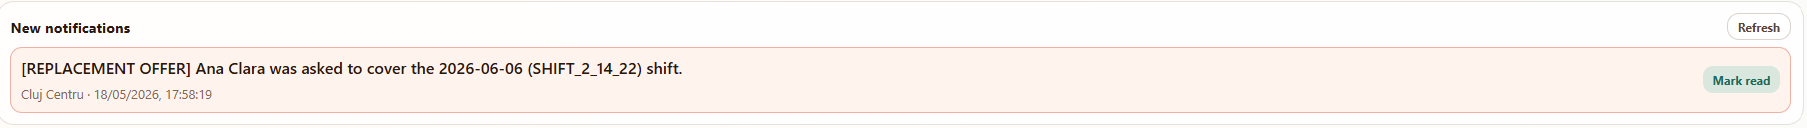
\includegraphics[width=1\linewidth]{ReplacementOffer2.png}
    \caption{Replacement offer flow - acknowledge phase 2}
    \label{fig:placeholder2}
\end{figure}

\begin{figure}[!h]
    \centering
    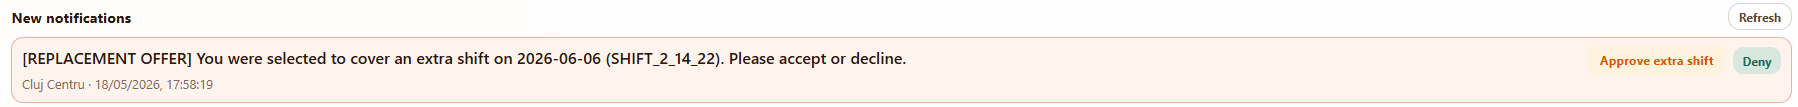
\includegraphics[width=1\linewidth]{ReplacementOffer3.png}
    \caption{Replacement offer flow - denial phase}
    \label{fig:placeholder3}
\end{figure}

\begin{figure}[!h]
    \centering
    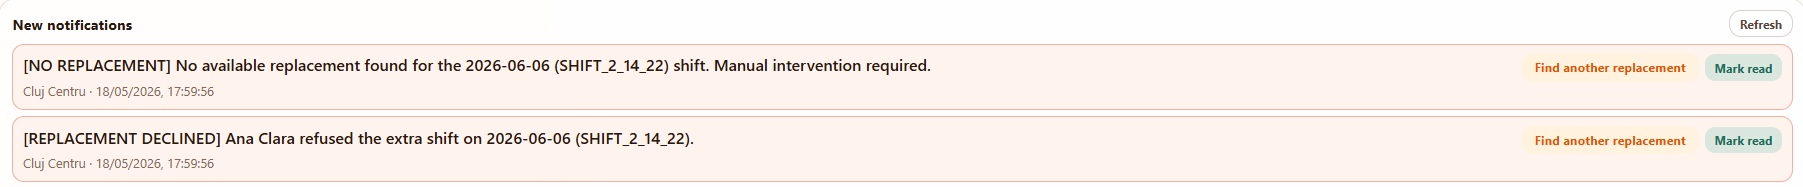
\includegraphics[width=1\linewidth]{ReplacementOffer4.png}
    \caption{Replacement offer flow - no replacement phase}
    \label{fig:placeholder4}
\end{figure}

%===========================================================
\section{Manual Operations and Schedule Adaptability}
\label{sec:manual_operations_and_schedule_adaptability}
%===========================================================

\subsection{Leave request flow}
\par The leave request system handles planned employee absences through a structured approval workflow that integrates directly with the scheduling and balance tracking subsystems.

\par Employees can submit leave requests for the second next calendar month only. This restriction is intentional: the scheduling algorithm runs a month at a time, for the next month, and confining leave requests to the upcoming month ensures that approved absences can be incorporated before the schedule is generated. Requests targeting past dates or the current month are rejected with an explicit error.

\par Before a request is accepted, the system validates several conditions:

\begin{itemize}
    \item The requesting user must be an employee (managers and administrators cannot submit leave requests through this endpoint).
    \item The requested date range must not overlap with any existing pending or approved leave request for the same employee, preventing double-booking of absence periods.
    \item The employee must have a positive remaining leave day balance; exhausted balances are reported to the employee with a suggestion to contact the manager directly.
    \item The number of calendar days requested must not exceed the remaining balance after accounting for the deductible day calculation.
\end{itemize}

\par The deductible day calculation applies a factor of 5/7 to the number of calendar days, reflecting the convention that only working days count against the leave balance. The result is rounded up to the nearest integer. For example, requesting seven calendar days deducts five leave days from the balance. This calculation is disclosed to the employee in the notification they receive after submitting the request. This measure is taken due to the special working hours that our stores use, from 10:00 to 22:00 each day of the week, leaving no free weekend days like in most of the other businesses.

\par Once the request is created, a \texttt{[LEAVE REQUEST]} notification is sent to the store manager, including the employee's name, the requested date range, the total calendar days, and the deductible count. The manager can then approve or deny the request directly from the notifications page.

\vspace{1.5em}
\begin{table}[h!]
    \centering
    \renewcommand{\arraystretch}{1.5} % Adds breathing room between rows
    \begin{tabular}{|l|p{6cm}|p{6cm}|}
        \hline
        \textbf{Action / Impact} & \textbf{Leave Approval} & \textbf{Leave Denial} \\ \hline
        \textbf{Entity Status} & Marked as \texttt{APPROVED} & Marked as \texttt{DENIED} \\ \hline
        \textbf{Data Logged} & Decision timestamp recorded & Optional textual reason stored on the entity \\ \hline
        \textbf{Leave Balance} & Deductible day count is subtracted & No change \\ \hline
        \textbf{Scheduling Engine} & Employee excluded from generation; zero shifts assigned during leave period & Standard scheduling applies \\ \hline
        \textbf{Notifications} & Confirmation sent to both the Manager (audit) and the Employee & Rejection sent to the Employee (including the reason if provided) \\ \hline
        \textbf{Follow-Up Action} & UI offers the Manager a "Regenerate month" action to fill newly vacant slots & None \\ \hline
    \end{tabular}
    \caption{Comparison of system actions based on the manager's leave request decision.}
    \label{tab:leave_decision_matrix}
\end{table}
\vspace{1.5em}

\subsection{Manual shift management}
\par Automated schedule generation covers the majority of operational cases, but real-world retail frequently requires targeted adjustments that fall outside the standard scheduling cycle. To address this, the system provides a manual shift management interface accessible to managers.

\subsubsection*{Adding a shift manually}
\par Managers can add individual shifts by selecting an employee, a date, and a shift type from the calendar interface. Before the shift is created, the backend applies the same constraint validation used by the automatic scheduler.

\begin{figure}[!h]
    \centering
    \begin{tikzpicture}[
        node distance=0.7cm,
        startbox/.style={rectangle, draw=blue!70, thick, fill=blue!5, text width=8.5cm, align=center, rounded corners=1ex, minimum height=0.8cm, font=\sffamily\bfseries},
        processbox/.style={rectangle, draw=black!70, thick, fill=gray!5, text width=8.5cm, align=left, rounded corners=1ex, minimum height=0.9cm, font=\sffamily\small},
        failbox/.style={rectangle, draw=red!70, thick, fill=red!5, text width=2.5cm, align=center, rounded corners=1ex, minimum height=0.8cm, font=\sffamily\footnotesize\bfseries},
        successbox/.style={rectangle, draw=green!70, thick, fill=green!5, text width=8.5cm, align=center, rounded corners=1ex, minimum height=0.8cm, font=\sffamily\bfseries},
        arrow/.style={thick, ->, >=stealth, draw=black!70},
        failarrow/.style={thick, ->, >=stealth, draw=red!70}
    ]

    % Nodes
    \node (start) [startbox] {Manual Shift Assignment Request};
    
    \node (step1) [processbox, below=0.8cm of start] {\textbf{1. Context Verification} \\ Verify that the targeted employee belongs strictly to the requesting manager's store.};
    
    \node (step2) [processbox, below=of step1] {\textbf{2. Eligibility Engine Execution} \\ Invoke \texttt{getEligibleEmployees} to rebuild tracker state and apply hard constraints: \\ 
    $\bullet$ Consecutive-day \& Weekly-hour limits \\ 
    $\bullet$ 12-hour back-to-back prohibition \\ 
    $\bullet$ Approved leave validation \\ 
    $\bullet$ Duplicate scheduling prevention};
    
    \node (step3) [processbox, below=of step2] {\textbf{3. Candidate Inclusion Check} \\ Verify that the specified employee exists within the newly generated eligible candidate set.};
    
    \node (step4) [processbox, below=of step3] {\textbf{4. Final Overlap Guard} \\ Perform a final validation to ensure the employee is not already assigned a shift on the target date.};
    
    \node (success) [successbox, below=0.8cm of step4] {Assignment Approved \& Persisted};

    % Fail Nodes
    \node (fail1) [failbox, right=1cm of step1] {Rejected};
    \node (fail2) [failbox, right=1cm of step2] {Rejected};
    \node (fail3) [failbox, right=1cm of step3] {Rejected};
    \node (fail4) [failbox, right=1cm of step4] {Rejected};

    % Pass Arrows
    \draw [arrow] (start) -- (step1);
    \draw [arrow] (step1) -- node[left, font=\sffamily\footnotesize] {Pass} (step2);
    \draw [arrow] (step2) -- node[left, font=\sffamily\footnotesize] {Pass} (step3);
    \draw [arrow] (step3) -- node[left, font=\sffamily\footnotesize] {Pass} (step4);
    \draw [arrow] (step4) -- node[left, font=\sffamily\footnotesize] {Pass} (success);

    % Fail Arrows
    \draw [failarrow] (step1.east) -- node[above, font=\sffamily\footnotesize] {Fail} (fail1.west);
    \draw [failarrow] (step2.east) -- node[above, font=\sffamily\footnotesize] {Fail} (fail2.west);
    \draw [failarrow] (step3.east) -- node[above, font=\sffamily\footnotesize] {Fail} (fail3.west);
    \draw [failarrow] (step4.east) -- node[above, font=\sffamily\footnotesize] {Fail} (fail4.west);

    \end{tikzpicture}
    \caption{Sequential validation and constraint pipeline for manual shift assignments.}
    \label{fig:manual_assignment_pipeline}
\end{figure}

\par If all checks pass, the shift is persisted with status \texttt{SCHEDULED} and the employee receives a \texttt{[NEW SHIFT]} notification informing them of the new assignment.

\par The frontend supports this flow by first calling a dedicated eligibility endpoint that returns the pre-filtered list of eligible employees for a given date and shift type. This allows the UI to populate the employee selector only with valid choices, providing a guided experience for the manager and eliminating the possibility of selecting an ineligible employee before the form is submitted.

\subsubsection*{Deleting a shift}
\par Managers can delete individual shifts directly from the calendar. The backend verifies that the shift belongs to the manager's store before proceeding with the deletion. Upon deletion, the affected employee receives a \texttt{[SHIFT REMOVED]} notification informing them that the assignment has been cancelled.

\par Shift deletion does not automatically trigger a replacement search intentionally, since the removal is typically an intentional managerial correction rather than an unexpected absence. If the manager needs to fill the vacated slot, they can use the manual add flow described above.

\subsection{Regeneration and data consistency during schedule updates}
\par Managers can regenerate the schedule for the next calendar month at any time. The most common scenarios are: a new employee is added to the store, a sales forecast file is updated with revised projections, or the manager simply wants to recalculate in case of a special occasion.

\par A critical correctness concern is that existing shifts may have linked absence requests, which in turn may have linked replacement offers. Deleting shifts without first removing these child records violates foreign key constraints at the database level. The regeneration logic therefore executes a cascading cleanup: it first identifies all absence request IDs linked to the shifts being removed, then deletes all replacement offers referencing those absence requests, then deletes the absence requests themselves, and finally deletes the shifts. This strict ordering ensures transactional integrity without requiring cascading deletes to be configured at the schema level, which would make the deletion behavior less visible in application code.

\par Additionally, the algorithm is specifically engineered to keep the approved leave requests in case of an emergency, therefore employees are not required to request again. This happens by keeping a \texttt{LeaveMap} function, which preserves the LeaveRequests table in the database, and freshly fetches the data for the specific month upon the time of re-generation. Instead of the scheduling algorithm constantly asking the database who is on vacation each day, it only asks the database once, builds this dictionary, and holds it in memory for the O(1) lookups.

\begin{figure}[!h]
    \centering
    
\includegraphics[width=1\linewidth]{figures/LeaveMap.png}
    \caption{buildLeaveMapFunction}
    \label{fig:placeholder_leavemap}
\end{figure}

%===========================================================
\section{System Integration and Communication}
\label{sec:system_integration_and_communication}
%===========================================================

\subsection{Notification system design}
\par All inter-role communication in QuickShift is mediated through a structured notification system. Each \texttt{Notification} entity stores a message string, the target user, the associated store, a read flag, and up to three optional foreign key references: a related absence request ID, a related leave request ID, and a related replacement offer ID.

\par These references allow the frontend to determine the action buttons to render for each notification without embedding workflow logic in the message text. The notification type is instead inferred from the message prefix (\texttt{[ABSENCE REQUEST]}, \texttt{[LEAVE REQUEST]}, \texttt{[REPLACEMENT OFFER]}, \texttt{[NO REPLACEMENT]}, and so on), which keeps the message human-readable while still being machine-parseable.

\par Notifications are marked as read in three ways: explicitly by the user clicking a read action, automatically after the user successfully completes the associated workflow action, or as a side effect of loading a new notification list after a successful operation. This multi-path read mechanism ensures that notifications do not linger after their workflow is complete, while also allowing managers to dismiss informational alerts that require no further action.

\begin{figure}[!h]
    \centering
    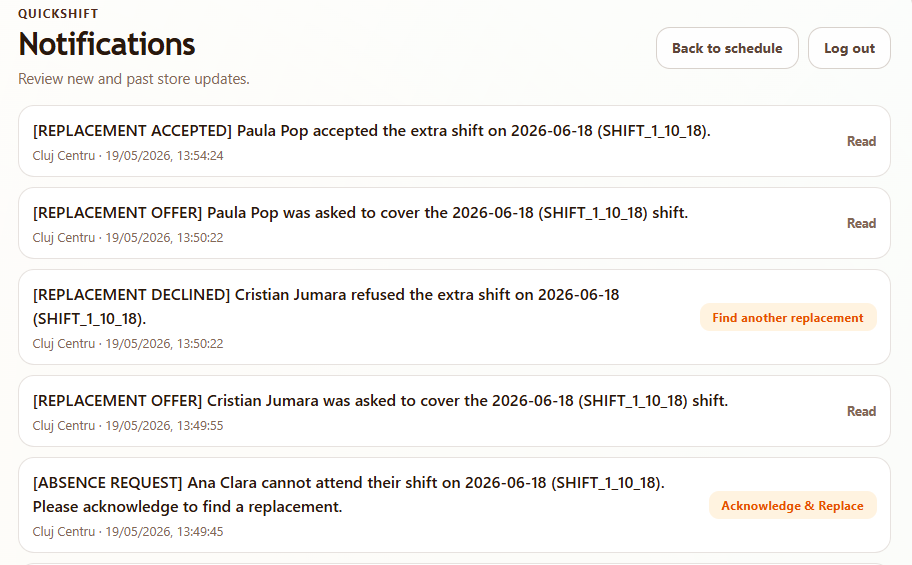
\includegraphics[width=0.7\linewidth]{NotificationPage.png}
    \caption{Notification Page design}
    \label{fig:placeholder_notif}
\end{figure}

\subsection{Complexity and practical performance considerations}
\par The main scheduling algorithm runs in $O(D \times E)$ time, where $D$ is the number of forecast days in the month and $E$ is the number of employees in scope. For typical retail stores with 30 forecast days and a team of five to fifteen employees, this is practically instantaneous.

\par The replacement algorithm has a higher constant factor because it performs a historical replay of all shifts from the beginning of the month to the absence date. The replay itself is $O(D' \times E)$ where $D'$ is the number of days elapsed in the month. However, this operation is triggered only on-demand and for a single absence event, so its cost is not on the critical path of normal scheduling operations.

\par The eligibility check for manual shift addition follows the same replay approach and has the same cost profile. Because it is user-initiated and operates on a single date, the response time is dominated by the database query rather than the computation, and is imperceptible to the user in practice.

\par By combining a fast, batch-oriented scheduling algorithm with targeted on-demand constraint checks for individual events, the implementation achieves a performance profile that is appropriate for interactive web use without requiring caching or background pre-computation.

%===========================================================
\section{Evaluation and Testing Approach}
\label{sec:evaluation_and_testing_approach}
%===========================================================

\par The system was evaluated through a multi-tiered approach, combining automated unit and integration testing with operational scenario validation. At the foundational level, a comprehensive suite of unit tests isolated and verified core business rules, while integration tests validated complex database queries and component interactions. Building upon this automated foundation, functional testing focused on verifying that the scheduler respects hard constraints across a range of forecast inputs: teams at or below the consecutive-day limit, teams with a mix of contract types, months containing approved leave, and months where sales forecasts cross both thresholds. In all tested scenarios, the generated schedule respected every hard constraint.

\par The replacement workflow was evaluated by simulating absence reports on various shift types and team compositions, including cases where the employee pool was small enough that some offers would be declined and the chain would need to proceed through multiple candidates. The auto-replacement logic correctly excluded previously declined employees in each retry and correctly identified the \texttt{UNRESOLVABLE} state when the pool was exhausted.

\par The leave request validation logic was rigorously tested for boundary conditions via integration tests targeting the database layer. These tests verified requests targeting the first and last days of the next month, requests that exactly exhaust the remaining balance, requests from employees with zero remaining balance, and precisely evaluated custom queries designed to detect all partial and total date overlaps with existing approved leave. All boundary cases produced the expected outcome.

\par To guarantee runtime auditability and facilitate real-time monitoring of complex business heuristics, a comprehensive application logging architecture was integrated using the SLF4J facade backed by the Logback framework. The system now contains over 50 strategic logging statements distributed across controllers, services, and database seeders. These logging calls are separated by severity levels to optimize performance and readability: the \texttt{INFO} level records key operational milestones (such as schedule generation runs, absence acknowledgments, and leave approval transitions), the \texttt{WARN} level captures validation failures and constraint breaches (such as role rejections or shift overlaps), and the \texttt{DEBUG} level monitors high-frequency polling events to prevent console noise. To ensure optimal execution efficiency, all log messages use SLF4J parameterized syntax (e.g., \texttt{log.info("...", arg)}), avoiding runtime string concatenation overhead unless the specific log level is active. This robust logging network provides developers and system administrators with absolute visibility into the execution flow of the CSP scheduler and the state machine transitions of the absence replacement engine.

\par User-facing evaluation focused on the click count and clarity of feedback for the most frequent workflows: generating a schedule, acknowledging an absence, approving a leave request, and adding a manual shift. Each of these workflows was designed to complete in three or fewer interactions from the point of recognizing the need for the action.